\documentclass[a4paper,12pt,obeyspaces,spaces,hyphens]{article}

\def \trainingtitle{Embedded Linux development with Buildroot training}
\def \trainingtype{online}
\def \trainingduration{5}
\def \agendalanguage{english}
\def \training{buildroot}

\usepackage{agenda}

\begin{document}

\feshowtitle

\feagendasummaryitem{Title}{
  {\bf \trainingtitle{}}
}
\feagendasummaryitem{Training objectives}{
  \begin{itemize}
  \item Be able to understand the role and principle of an embedded
    Linux build system, and compare Buildroot to other tools offering
    similar functionality.
  \item Be able to create a simple embedded Linux system with
    Buildroot: create a configuration, run the build, install the
    result on an embedded platform.
  \item Be able to adjust the Buildroot configuration to build an
    embedded Linux system tailored to specific needs: choice of the
    cross-compilation toolchain, management of the Linux kernel
    configuration, customization of the root filesystem contents, etc.
  \item Be able to create new packages in Buildroot to integrate
    additional applications and libraries into the embedded Linux
    system.
  \item Be able to use the tools offered by Buildroot to manage and
    analyze the build: security vulnerability tracking, license
    compliance, etc.
  \item Be able to develop and debug Linux user-space applications in
    the context of Buildroot.
  \item Be able to interact with the Buildroot open-source community,
    and to understand the internals of Buildroot.
  \end{itemize}
}
\feagendasummaryitem{Duration}{
  {\bf Five} half days - 20 hours (4 hours per half day).
}
\onlinepedagogics{buildroot}
\feagendasummaryitem{Trainer}{
  One of the engineers listed on:
  \newline \url{https://bootlin.com/training/trainers/}
}
\feagendasummaryitem{Language}{
  Oral lectures: English
  \newline Materials: English.
}
\feagendasummaryitem{Audience}{
  Companies already using or interested in using
  Buildroot to build their embedded Linux systems.
}
\feagendasummaryitem{Prerequisites}{
  \begin{itemize}
    \prerequisitecommandline
    \prerequisiteembeddedlinux
    \prerequisiteenglish
  \end{itemize}
}
\feagendasummaryitem{Required equipment}{
  \begin{itemize}
  \item Computer with the operating system of your choice, with the
    Google Chrome or Chromium browser for videoconferencing.
  \item Webcam and microphone (preferably from an audio headset)
  \item High speed access to the Internet
  \end{itemize}
}
\certificate{}
\disabilities{}

\feagendatwocolumn
{Hardware platform for practical labs, option \#1}
{
  {\bf BeagleBone Black} board
  \begin{itemize}
  \item An ARM AM335x (single Cortex-A8) processor from Texas
    Instruments
  \item USB powered
  \item 512 MB of RAM
  \item 2 or 4 GB of on-board eMMC storage
  \item USB host and device
  \item HDMI output
  \item 2 x 46 pins headers, to access UARTs, SPI buses, I2C buses
    and more.
  \end{itemize}
}
{}
{
  \begin{center}
    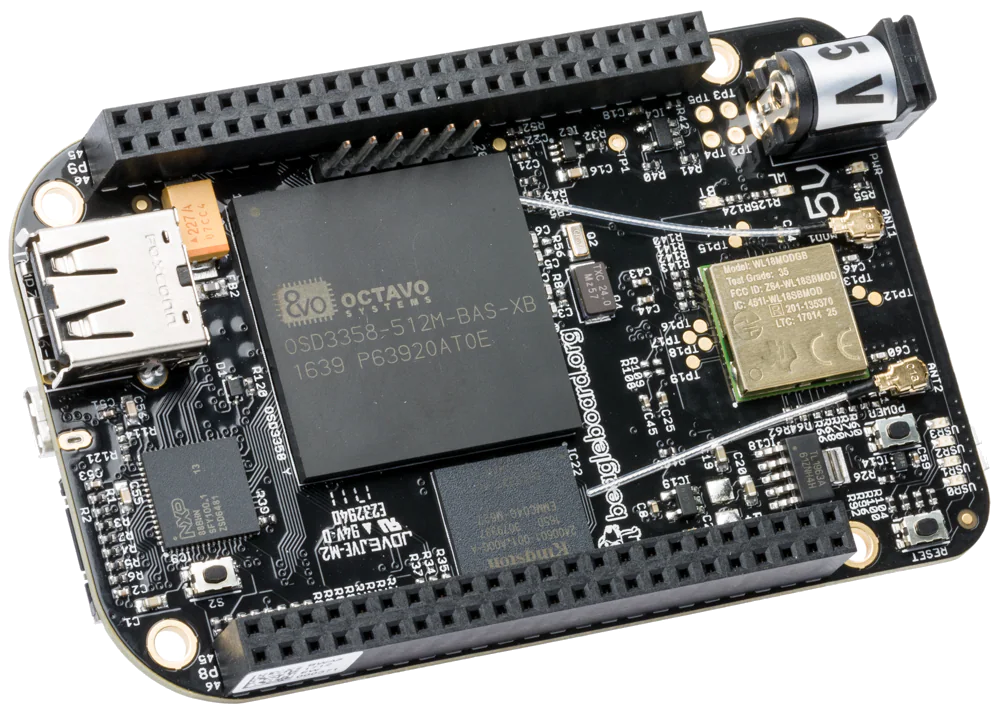
\includegraphics[width=5cm]{../slides/beagleboneblack-board/beagleboneblack.png}
  \end{center}
}

\feagendatwocolumn
{Hardware platform for practical labs, option \#2}
{
  {\bf STMicroelectronics STM32MP157D Discovery Kit~1} board
  \begin{itemize}
  \item STM32MP157D (dual Cortex-A7) processor from STMicroelectronics
  \item USB powered
  \item 512 MB DDR3L RAM
  \item Gigabit Ethernet port
  \item 4 USB 2.0 host ports
  \item 1 USB-C OTG port
  \item 1 Micro SD slot
  \item On-board ST-LINK/V2-1 debugger
  \item Arduino compatible headers
  \item Audio codec, buttons, LEDs
  \end{itemize}
}
{}
{
  \begin{center}
    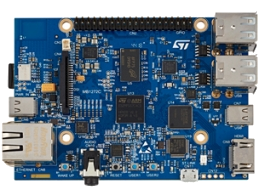
\includegraphics[width=5cm]{../slides/discovery-board-dk1/discovery-board-dk1.png}
  \end{center}
}

\section{Half day 1}

\feagendatwocolumn
{Lecture - Embedded Linux and build system introduction}
{
  \begin{itemize}
  \item The general architecture of an embedded Linux system
  \item Build systems vs. binary distributions
  \item Role of a build system
  \item Comparison of existing build systems
  \end{itemize}
}
{Lecture - Introduction to Buildroot}
{
  \begin{itemize}
  \item Key facts about the project
  \item Getting Buildroot
  \item Basic configuration of Buildroot
  \item Doing a first build
  \end{itemize}
}
\\
\feagendatwocolumn
{Demo - Basic Buildroot usage}
{
  \begin{itemize}
  \item Getting and setting up Buildroot
  \item Configuring and building a basic system with Buildroot for an
    embedded platform
  \item Flash and test the generated system
  \end{itemize}
}
{Lecture - Managing the build and configuration}
{
  \begin{itemize}
  \item Out of tree build
  \item Using and creating {\em defconfigs}
  \item Defconfig fragments
  \item Other building tips
  \end{itemize}
}

\feagendaonecolumn
{Lecture - Buildroot source and build trees}
{
  \begin{itemize}
  \item Details about the Buildroot source code organization
  \item Details about the Buildroot build tree
  \end{itemize}
}


\section{Half day 2}

\feagendaonecolumn
{Lecture - Toolchains in Buildroot}
{
  \begin{itemize}
  \item The different choices for using toolchains in Buildroot
  \item Overview of the toolchain options
  \item Using existing binary toolchains, such as Bootlin
    toolchains, understanding {\em multilib} capabilities and
    integration of toolchains in Buildroot
  \item Generating custom toolchains with {\em Crosstool-NG}, and
    re-use them as external toolchains
  \end{itemize}
}

\feagendatwocolumn
{Lecture - Managing the Linux kernel configuration}
{
  \begin{itemize}
  \item Loading, changing and saving the kernel configuration
  \end{itemize}
}
{Lecture - Root filesystem construction in Buildroot}
{
  \begin{itemize}
  \item Understand how Buildroot builds the root filesystem: {\em
      skeleton}, installation of packages, overlays, {\em post-build}
    and {\em post-image} scripts.
  \item Customization of the root filesystem contents
  \item System configuration: {\em console} selection, various {\tt
      /dev} management methods, the different {\tt init}
    implementations, etc.
  \item Understand how Buildroot generates filesystem images
  \end{itemize}
}

\feagendaonecolumn
{Demo - Root filesystem customization}
{
  \begin{itemize}
  \item Explore the build output
  \item Customize the root filesystem using a {\em rootfs overlay}
  \item Customize the kernel with patches and additional configuration
    options
  \item Add more packages
  \item Use {\em defconfig} files and {\em out of tree} build
  \end{itemize}
}

\feagendaonecolumn
{Lecture - Download infrastructure in Buildroot}
{
  \begin{itemize}
  \item Downloading logic
  \item Primary site and backup site, doing offline builds
  \item VCS download, integrity checking
  \item Download-related {\em make} targets
  \end{itemize}
}

\section{Half day 3}

\feagendaonecolumn
{Lecture - GNU Make 101}
{
  \begin{itemize}
  \item Basics of make rules
  \item Defining and referencing variables
  \item Conditions, functions
  \item Writing recipes
  \end{itemize}
}

\feagendatwocolumn
{Lecture - Integrating new packages in Buildroot}
{
  \begin{itemize}
  \item How to integrate new packages in the Buildroot configuration
    system
  \item Understand the different package infrastructures: for {\em
      generic}, {\em autotools}, {\em CMake}, {\em Python} packages
    and more.
  \item Writing a package \code{Config.in} file: how to express
    dependencies on other packages, on toolchain options, etc.
  \item Details on writing a package recipe: describing the package
    source code location, download method, configuration, build and
    installation steps, handling dependencies, etc.
  \end{itemize}
}
{Demo - New packages in Buildroot}
{
  \begin{itemize}
  \item Create a new package for {\em nInvaders}
  \item Understand how to add dependencies
  \item Add patches to {\em nInvaders} for {\em Nunchuk} support
  \end{itemize}
}

\feagendaonecolumn
{Lecture - Advanced package aspects}
{
  \begin{itemize}
  \item Licensing report
  \item Patching support: patch ordering and format, global patch directory, etc.
  \item User, permission, device tables
  \item Init scripts and systemd unit files
  \item Config scripts
  \item Understanding {\em hooks}
  \item Overriding commands
  \item Legacy handling
  \item Virtual packages
  \end{itemize}
}

\section{Half day 4}

\feagendaonecolumn
{Demo - Advanced packages}
{
  \begin{itemize}
  \item Package an application with a mandatory dependency and an
    optional dependency
  \item Package a library, hosted on GitHub
  \item Use {\em hooks} to tweak packages
  \item Add a patch to a package
  \end{itemize}
}

\feagendaonecolumn
{Lecture - Analyzing the build: licensing, dependencies, build time}
{
  \begin{itemize}
  \item Usage of the legal information infrastructure
  \item Graphing dependencies of packages
  \item Collecting and graphing build time information
  \end{itemize}
}

\feagendatwocolumn
{Lecture - Advanced topics}
{
  \begin{itemize}
  \item \code{BR2_EXTERNAL} to store customizations outside of the
    Buildroot sources
  \item Package-specific targets
  \item Understanding rebuilds
  \item Tips for building faster
  \end{itemize}
}
{Demo - Advanced aspects}
{
  \begin{itemize}
  \item Use build time graphing capabilities
  \item Use dependency graphing capabilities
  \item Use licensing report generation, and add licensing
    information to your own packages
  \item Use \code{BR2_EXTERNAL}
  \end{itemize}
}

\newpage

\section{Half day 5}

\feagendatwocolumn
{Lecture - Application development with Buildroot}
{
  \begin{itemize}
  \item Using Buildroot during application development
  \item Usage of the Buildroot environment to build applications
    outside of Buildroot
  \item Generate an SDK for other developers
  \item Remote debugging with Buildroot
  \end{itemize}
}
{Demo - Application development with Buildroot}
{
  \begin{itemize}
  \item Build and run your own application
  \item Remote debug your application
  \item Use \code{<pkg>_OVERRIDE_SRCDIR}
  \end{itemize}
}

\feagendatwocolumn
{Lecture - Understanding Buildroot internals}
{
  \begin{itemize}
  \item Detailed description of the Buildroot build process:
    toolchain, packages, root filesystem construction, stamp files,
    etc.
  \item Understanding virtual packages.
  \end{itemize}
}
{Lecture - Getting support and contributing}
{
  \begin{itemize}
  \item Getting support: {\em Bugzilla}, {\em mailing list}, {\em IRC}
  \item Contributing: understanding the development process, how to
    submit patches
  \end{itemize}
}

\feagendaonecolumn
{Questions and Answers}
{
  \begin{itemize}
  \item Questions and answers with the audience about the course topics
  \item Extra presentations if time is left, according what most
        participants are interested in.
  \end{itemize}
}

Note: the last session might be shorter than the other sessions and
finish earlier, depending on the progress and questions from the
participants.

\end{document}
